\documentclass[11pt]{article}
\usepackage[T1]{fontenc}
\usepackage[utf8]{inputenc}
\usepackage[a4paper,margin=25mm]{geometry}
\usepackage{amsmath,amssymb,amsthm,booktabs,graphicx,microtype,xcolor}
\usepackage[colorlinks=true,linkcolor=teal!70!black,urlcolor=teal!70!black,citecolor=teal!70!black]{hyperref}
\newtheorem{theorem}{Theorem}
\newtheorem{proposition}[theorem]{Proposition}
\newtheorem{corollary}[theorem]{Corollary}
\theoremstyle{remark}\newtheorem{remark}[theorem]{Remark}
\newcommand{\Mell}{\mathcal M}
\newcommand{\Res}{\operatorname{Res}}
\setlength{\parindent}{0pt}
\setlength{\parskip}{5pt}
\title{Infrared Identifiability in Celestial Mellin Space}
\author{\normalsize Deep Bhattacharjee, James Montgomery Lockwood, Tristan Romanov,\\
\normalsize Ikailo John Sessford, Ushashi Bhattacharya, Sanjeevan Singha Roy}
\date{Working research draft, 15 November 2026}
\begin{document}
\maketitle
\begin{center}\small\color{teal!70!black}
One unranked prospective author list supplied by the project lead.\\
Coauthor review and approval remain pending.
\end{center}
\begin{abstract}
We study the stability of extracting soft data from scalar celestial Mellin kernels. An explicit family of positive profiles, all analytic in the same complex disc after removing their prescribed soft power, has a fixed soft residue while its Mellin transforms converge uniformly to zero on an entire vertical line. We calculate the exact norm and its decay. Under a fixed-order polynomial-log assumption, we then obtain the sharp deterministic noise amplification for the highest Mellin pole coefficient from a finite logarithmic energy interval. Finally, we derive the transformation of pole coefficients under local energy-unit changes and show how a transforming reference energy cancels the additional Mellin weight. The arguments use classical beta integrals, Chebyshev extremality, and scale covariance. Originality of the combined celestial formulation remains under review. Application to a full scattering theory requires additional physical assumptions.
\end{abstract}

\section{Question and mathematical setting}
The celestial basis replaces energy variables by Mellin weights. Soft expansions then appear as poles of a meromorphic continuation. Pasterski's chapter gives this dictionary and notes that loops can generate higher poles \cite{pasterski}. Perimeter's initiative motivates connecting scattering data with the resulting boundary structures \cite{perimeter}. The issue studied here is whether an accurate transform gives accurate soft data.

For a scalar kernel $A$ on $(0,\infty)$, set
\begin{equation}\label{eq:mellin}
 \Mell A(s)=\int_0^\infty \omega^{s-1}A(\omega)\,d\omega
\end{equation}
in its absolute-convergence strip, followed by meromorphic continuation when available. All energies in this expression are numerical values in a chosen unit. Section~\ref{sec:units} treats the reference convention explicitly.

The results concern scalar kernels at fixed remaining kinematic parameters. Their hypotheses do not impose the complete set of constraints of a unitary crossing-symmetric $S$-matrix. Establishing an appropriate physical subclass is a separate research step. The finite-log result applies at a fixed perturbative order. Gu, Li, and Wang show that resummation can instead produce branch cuts \cite{gu}.

\section{A fixed residue with vanishing complete line data}
\begin{theorem}[Exact instability family]\label{thm:instability}
Fix $R>0$, $c>0$, $p\in\mathbb R$, and $a>0$. For integers $N>a$, define
\begin{equation}\label{eq:family}
 A_N(\omega)=c\omega^{-p}(1+\omega/R)^{-N}.
\end{equation}
Then its Mellin transform converges for $p<\Re s<p+N$ and equals
\begin{equation}\label{eq:beta}
 F_N(s)=cR^{s-p}B(s-p,N-s+p).
\end{equation}
Its continuation has residue $c$ at $s=p$, whereas
\begin{equation}\label{eq:exactnorm}
 \sup_{\nu\in\mathbb R}|F_N(p+a+i\nu)|
 =cR^a B(a,N-a)
 \sim cR^a\Gamma(a)N^{-a}\longrightarrow0.
\end{equation}
The stripped profiles $(1+\omega/R)^{-N}$ are positive and completely monotone on $(0,\infty)$. Each has complex analyticity radius exactly $R$ at zero.
\end{theorem}
\begin{proof}
Substitute $x=\omega/R$ into \eqref{eq:mellin} and use the beta integral \cite{dlmfbeta}. At $s=p+z$, the identity
\[
 F_N(p+z)=cR^z\frac{\Gamma(z)\Gamma(N-z)}{\Gamma(N)}
\]
has residue $c$ at $z=0$. On $\Re z=a$, the absolute value of the defining integral is at most
\[
 cR^a\int_0^\infty x^{a-1}(1+x)^{-N}\,dx.
\]
Equality holds at $\Im z=0$, proving the exact supremum. The standard gamma-ratio asymptotic yields the limit in \eqref{eq:exactnorm}. Alternatively, its vanishing alone follows by dominated convergence after fixing one integer $N_0>a$.

For every $k\ge0$,
\[
 (-1)^k\frac{d^k}{d\omega^k}(1+\omega/R)^{-N}
 =\frac{(N)_k}{R^k}(1+\omega/R)^{-N-k}>0.
\]
Here $(N)_k$ is a rising factorial. For integer $N$, the stripped rational function has its nearest singularity at $-R$, a pole of order $N$. Its Taylor radius is therefore $R$ for every member of the family.
\end{proof}

\begin{corollary}[Failure of continuous residue recovery]\label{cor:discontinuous}
On the class consisting of zero and the family in Theorem~\ref{thm:instability}, residue extraction at $p$ is discontinuous for the norm $\|F\|_{a,\infty}=\sup_\nu|F(p+a+i\nu)|$. For any error tolerance $\eta>0$, some pair with residues $0$ and $c$ admits the same line data up to uniform error $\eta$. Every reconstruction rule then has worst-case residue error at least $c/2$ on that pair.
\end{corollary}
\begin{proof}
Choose $N$ so large that $\|F_N\|_{a,\infty}\le2\eta$. The common observation $F_N/2$ is within $\eta$ of both zero and $F_N$. An estimate cannot be closer than $c/2$ to both residues.
\end{proof}

Discontinuity also holds within a class consisting entirely of strictly positive profiles with Taylor radius exactly $R$. Fix $d>0$ and an integer $N_0>a$, and take $B(\omega)=d\omega^{-p}(1+\omega/R)^{-N_0}$. The kernels $B+A_N$ converge to $B$ in the line-data norm, while their residues are $d+c$ and $d$. Their stripped profiles are completely monotone and have nearest singularity $-R$. The same midpoint-observation argument gives the error lower bound $c/2$.

When $a=1$ and $N>1$, the line norm is the elementary quantity $cR/(N-1)$. The first stripped derivative at zero is $-N/R$. Thus fixed analyticity radius and positivity allow the variation scale to shrink without a uniform derivative bound. The conclusion concerns stability under noisy data. Exact transform data on a line still determine each admissible kernel by the usual uniqueness theory.

\begin{figure}[ht]
\centering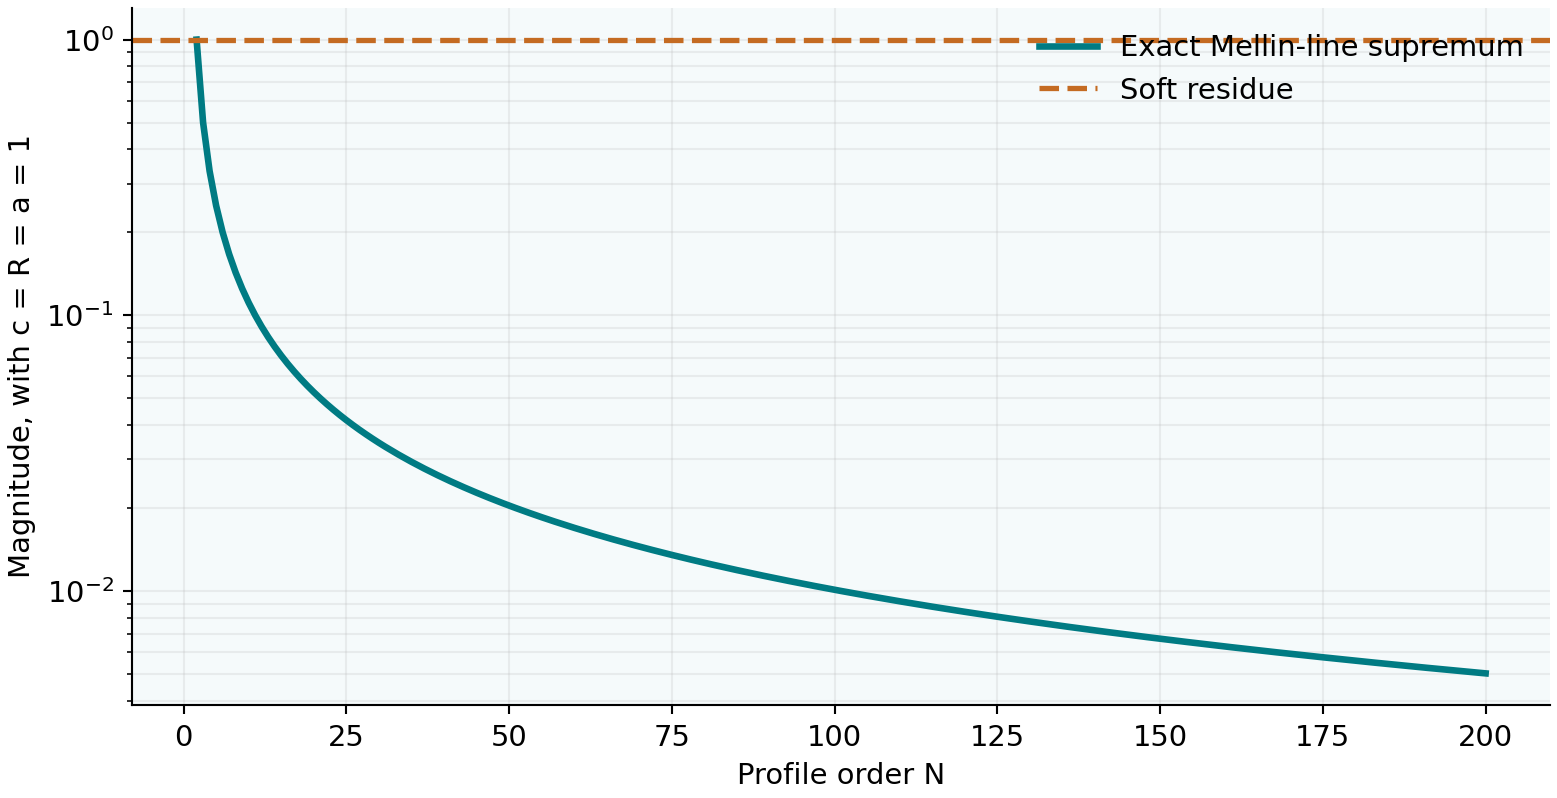
\includegraphics[width=.92\linewidth]{assets/residue-instability.png}
\caption{The exact line norm for $c=R=a=1$ is $1/(N-1)$, while the residue remains one. The profiles all have Taylor radius one.}
\end{figure}

\section{Optimal recovery under a fixed-order soft-log assumption}
This section assumes observations of the stripped kernel in energy space. Access to these observations is an additional data assumption beyond the Mellin-line norm in Section~2.
Set $t=\log(\mu/\omega)$ with a fixed reference energy $\mu>0$. Suppose an infrared kernel has the local form
\begin{equation}\label{eq:logansatz}
 A(\omega)=\omega^\kappa P(t),\qquad
 P(t)=\sum_{j=0}^m a_jt^j,\quad 0<\omega\le\mu.
\end{equation}
The ultraviolet Mellin integral of any completion considered here is assumed absolutely convergent in an open neighborhood of $s=-\kappa$, and hence holomorphic there. This also supplies a common convergence strip with the infrared integral. Direct integration gives
\begin{equation}\label{eq:polelog}
 \int_0^\mu \omega^{s+\kappa-1}P(\log(\mu/\omega))\,d\omega
 =\mu^{s+\kappa}\sum_{j=0}^m\frac{j!a_j}{(s+\kappa)^{j+1}}.
\end{equation}
The coefficient of the highest possible pole is consequently $m!a_m$. This scalar highest-pole coefficient is the recovery target. Lower coefficients of the principal part also receive terms from the analytic prefactor.
For observations from the infrared range in \eqref{eq:logansatz}, take $L\ge0$. The polynomial recovery theorem itself holds on any real interval.

\begin{theorem}[Sharp deterministic recovery]\label{thm:cheb}
Let $m\ge1$, $T>0$, and $L\in\mathbb R$. Observe $y=P+e$ on $[L,L+T]$, where $P$ is an arbitrary real polynomial of degree at most $m$ and $\|e\|_\infty\le\delta$. The minimax worst-case error for recovering $a_m$ is exactly
\begin{equation}\label{eq:kappa}
 \delta K_m,\qquad K_m=\frac{2^{2m-1}}{T^m}.
\end{equation}
An estimator using $m+1$ point values attains the optimum. In the setting \eqref{eq:logansatz}, the exact corresponding error for the highest pole coefficient is $\delta m!K_m$.
\end{theorem}
\begin{proof}
Take $x_j=\cos(j\pi/m)$ and $t_j=L+T(1+x_j)/2$ for $0\le j\le m$. In decreasing order, these are distinct. Define
\[
 w_j=\left(\prod_{k\ne j}(t_j-t_k)\right)^{-1}.
\]
The leading coefficient in the Lagrange interpolation formula is
\[
 a_m=\sum_{j=0}^m w_jP(t_j).
\]
The sign of $w_j$ is $(-1)^j$. The polynomial
\[
 Q(t)=T_m\left(\frac{2(t-L)}{T}-1\right)
\]
has values $(-1)^j$ at these nodes and leading coefficient $K_m$ by the classical Chebyshev identities \cite{dlmfcheb}. Applying the same interpolation formula to $Q$ gives $\sum_j|w_j|=K_m$. Therefore $\widehat a_m=\sum_jw_jy(t_j)$ has error at most $\delta K_m$.

For the matching lower bound, take $P_\pm=\pm\delta Q$. Both are compatible with the identical observation $y=0$ on the entire interval. Their leading coefficients are $\pm\delta K_m$. Every rule therefore has worst-case error at least $\delta K_m$. Multiplication by $m!$ proves the last assertion.
\end{proof}

\begin{proposition}[Controlled remainder]\label{prop:remainder}
Suppose instead $y=P+R+e$, with $|R(t)|\le Me^{-\alpha t}$ on $[L,L+T]$, $\alpha>0$, and $\|e\|_\infty\le\delta$. The estimator in Theorem~\ref{thm:cheb} satisfies
\[
 |\widehat a_m-a_m|\le K_m(\delta+Me^{-\alpha L}).
\]
The statement supplies an upper bound for this remainder class. It makes no joint optimality assertion for the two error terms.
\end{proposition}
\begin{proof}
At each sample point the combined perturbation is at most $\delta+Me^{-\alpha L}$. Apply the weight-sum identity.
\end{proof}

Interpreting the estimated coefficient as an actual infrared pole coefficient requires a condition beyond the observed interval. If $R$ is locally integrable and $|R(t)|\le Me^{-\alpha t}$ for all sufficiently large $t$, its infrared Mellin contribution is holomorphic in $\Re(s+\kappa)>-\alpha$. It then contributes no principal part at $s=-\kappa$. A bound confined to the observation window permits a smooth remainder that vanishes on that window and becomes $t^m$ farther into the infrared; that remainder changes the highest pole coefficient. Thus Proposition~\ref{prop:remainder} estimates a finite-window polynomial coefficient, and the stated tail condition supplies its pole interpretation.

A shift of reference energy translates $t$ and changes lower polynomial coefficients, while preserving $a_m$ and the interval width $T$. The recovery constant depends on this width. For $m=0$, direct recovery has error $\delta$.

\section{Local energy units and reference conventions}\label{sec:units}
Muntz develops a gauge-theoretic language for units \cite{muntz}. Here we explicitly distinguish a Mellin transform of numerical energy from one whose kernel includes a transforming reference energy. Let $x$ denote external coordinates and let $b(x,\omega)$ have ordinary unit weight $w$. For a smooth real $\sigma(x)$, set
\begin{equation}\label{eq:unitlaw}
 \omega'=e^{-\sigma(x)}\omega,\qquad
 b'(x,\omega')=e^{-w\sigma(x)}b(x,e^{\sigma(x)}\omega'),
 \qquad A'=A+d\sigma.
\end{equation}
The one-form $A$ describes the chosen comparison of units. First assume $b$ is smooth and compactly supported away from zero and infinity, locally uniformly in $x$.

\begin{theorem}[Mellin covariance and pole jets]\label{thm:units}
For $M_s=\int_0^\infty\omega^sb(x,\omega)\,d\omega/\omega$,
\begin{align}
 M_s'&=e^{-(w+s)\sigma}M_s,\label{eq:mellinunit}\\
 \Mell[(d_x-A\omega\partial_\omega+wA)b]
 &=[d_x+(w+s)A]M_s.\label{eq:connection}
\end{align}
These formulas also hold in a nonempty strip if $b$, $d_xb$, and $\omega\partial_\omega b$ have locally uniform integrable majorants on compact substrips and $\omega^sb\to0$ at both energy endpoints. They then hold wherever both sides admit meromorphic continuation. If that continuation has principal part $\sum_{j=1}^r a_{-j}(s-s_0)^{-j}$, then
\begin{equation}\label{eq:jet}
 a'_{-k}=e^{-(w+s_0)\sigma}
 \sum_{j=k}^r\frac{(-\sigma)^{j-k}}{(j-k)!}a_{-j},\qquad 1\le k\le r.
\end{equation}
In particular, the pole's location and order are preserved.
\end{theorem}
\begin{proof}
For \eqref{eq:mellinunit}, substitute $\omega=e^\sigma\omega'$. For \eqref{eq:connection}, integration by parts gives $\Mell[\omega\partial_\omega b]=-sM_s$. The stipulated boundary and differentiability conditions justify these operations. Expanding $e^{-(s-s_0)\sigma}$ and collecting negative Laurent powers proves \eqref{eq:jet}. Its top coefficient is multiplied by a nonzero factor, preserving the order.
\end{proof}

For example, when $w+s_0=0$ and the pole is double, $a'_{-2}=a_{-2}$ and $a'_{-1}=a_{-1}-\sigma a_{-2}$. Thus the ordinary residue generally changes even when the highest coefficient is neutral. Logarithmic celestial structures have established precedents \cite{bissi}; the displayed formula is an explicit convention calculation.

\begin{proposition}[Transforming reference energy]\label{prop:compensator}
Let $\mu'=e^{-\sigma}\mu$ and define $\widehat M_s=\mu^{-s}M_s$ using the dimensionless kernel $(\omega/\mu)^s$. Then
\begin{equation}
 \widehat M_s'=e^{-w\sigma}\widehat M_s.
\end{equation}
Every Laurent coefficient of $\widehat M$ has this same ordinary weight. Its change of energy unit induces no triangular mixing.
\end{proposition}
\begin{proof}
Multiply \eqref{eq:mellinunit} by $(\mu')^{-s}=e^{s\sigma}\mu^{-s}$ and collect Laurent coefficients. The transformation factor is independent of $s$.
\end{proof}

The numerical-energy jet can be written as an associated representation with generator $J=(w+s_0)I+N$, where $(Na)_{-k}=a_{-(k+1)}$ and the last component is zero. Its connection is $d+JA$ and its curvature is $J\,dA$. A pure unit choice $A=d\log u$ is flat. A nonzero curvature requires additional transport structure. Proposition~\ref{prop:compensator} shows why the extra Mellin charge by itself cannot establish a new physical gauge coupling.

\section{Interpretation, reproducibility, and open steps}
The instability theorem gives an exact counterexample to continuous residue recovery in a stated norm on a stated function class. It persists under fixed analyticity radius and complete monotonicity. The finite-window theorem gives a matching optimal estimator once a stronger finite-degree model is assumed. The unit calculation identifies precisely which pole coefficients depend on the numerical-energy convention.

Three issues remain for a broader physics claim. First, the instability family needs to be embedded into, or replaced by a family within, the desired physical scattering class. Second, using finite-order soft logarithms requires a justified remainder estimate and control of resummation. Third, a broader originality review must determine whether the combined results supply a new contribution beyond established inverse-problem and celestial literature. The present bounded search establishes extensive antecedents. Priority remains unresolved.

The repository includes exact rational and symbolic identities, an independent Julia replay, high-precision beta-integral comparisons, and negative controls. Finite executions check the implementations. The proofs above establish their stated generalizations. Computational records identify exact and numerical components separately.

\paragraph{Authorship and preparation.}
The six-person unranked byline was requested by the project lead and transcribed from the related Yang-Mills project's author record. Coauthor review, contribution statements, and approval of this manuscript remain pending. An AI coding assistant assisted derivation, literature search, coding, and drafting. Any submitting authors must review the work and take responsibility for the version they approve.

\begin{thebibliography}{9}
\bibitem{pasterski} S. Pasterski, \emph{A Chapter on Celestial Holography}, arXiv:2310.04932v2 (2023), \url{https://arxiv.org/abs/2310.04932v2}.
\bibitem{perimeter} Perimeter Institute, \emph{Celestial Holography Initiative}, accessed 15 November 2026, \url{https://perimeterinstitute.ca/research/research-centres-and-initiatives/celestial-holography-initiative}.
\bibitem{muntz} B. Muntz, \emph{Dimensional Analysis is a Gauge Theory}, arXiv:2607.21695v1 (2026), \url{https://arxiv.org/abs/2607.21695}.
\bibitem{gu} J. Gu, Y.-Y. Li, L.-T. Wang, \emph{A Note on the Analytic Structure of Celestial Amplitudes}, JHEP 08 (2022) 257, \url{https://arxiv.org/abs/2206.01757}.
\bibitem{bissi} A. Bissi, L. Donnay, B. Valsesia, \emph{Logarithmic doublets in CCFT}, arXiv:2407.17123 (2024), \url{https://arxiv.org/abs/2407.17123}.
\bibitem{dlmfbeta} NIST Digital Library of Mathematical Functions, \S5.12, \emph{Beta Function}, \url{https://dlmf.nist.gov/5.12}.
\bibitem{dlmfcheb} NIST Digital Library of Mathematical Functions, \S18.5, \emph{Explicit Representations}, \url{https://dlmf.nist.gov/18.5}.
\end{thebibliography}
\end{document}
